\chapter{State-Space Aggregation}\label{ch:lumping}
In this part, we propose a  method to identify a truncation that optimizes the trade-off between the size of the considered state-space and the approximation error due to the \acf{FSP}\turnto{sec:fsp}\@.
To this end, we start with a very coarse-grained model abstraction that we refine iteratively. 
The coarse-grained model is based on an grid-shaped aggregation (i.e.\ lumping) scheme that identifies a set of macro-states.
These macro-states can be used to compute an interim model solution that guides the refinement in the next step.
We perform refinements until the approximation arrives at the resolution of the original model (i.e.\ each macro-state has only one constituent) such that the aggregation introduces no approximation error.

\section{Macro-States}
A macro-state is a collection of micro-states (or simply states) treated as one state in the aggregated model, which can be seen as an abstraction of the original model.
The aggregation scheme defines a partitioning of the state-space.
We choose a scheme based on a grid structure. That is, each macro-state is a hypercube in $\mathbb{Z}_{\geq 0}^{n_S}$.

Hence, each macro-state $\bar{x}_i(\ell^{(i)},u^{(i)})$ (denoted by $\bar{x}_i$ for notational ease) can be identified using two vectors $\ell^{(i)}$
and $u^{(i)}$.
The vector $\ell^{(i)}$ gives the corner closest to the origin, while $u^{(i)}$
gives the corner farthest from the origin.
Formally,
\begin{equation}\label{eq:macro_state}
    \bar{x}_i = \bar{x}_i(\ell^{(i)},u^{(i)}) =  \{x\in\mathbb{N}^{n_S} \mid  \ell^{(i)}  \leq x  \leq u^{(i)} \},
\end{equation}
where '$\leq$' denotes element-wise comparison.

In order to solve the aggregated model, we need to define transition rates between macro-states.
Therefore, we assume that, given that the system is in a particular macro-state, all constituent states are equally likely (uniformity assumption).
This assumption is the reason why the aggregated model provides only a coarse-grained approximation. 

The uniformity assumption is a modeling choice yielding significant advantages.
Firstly, it eases the computation of the rates between macro-states and, therefore, makes a fast solution of the aggregated model possible.
Secondly, even though it induces an approximation error, it provides suitable guidance as uniformity assumption spreads out the probability mass conservatively.
Hence, it becomes less likely that regions of interest are disregarded.
Lastly, the uniformity assumption is theoretically well-founded, as it stems from the maximum entropy principle: 
In the absence of concrete knowledge about the probability distribution inside a macro-state, we assume the distribution with the highest uncertainty, i.e., the uniform distribution. 

\section{Construction}
The grid structure makes the computation of transition rates between macro-states particularly convenient and computationally simple.
Mass-action reaction rates can be given in a closed-form,
due to the Faulhaber formulae~\parencite{knuth1993johann} and more complicated rate functions such as Hill-functions can often be handled as well by taking appropriate integrals (see page~\pageref{model:hill_toggle}).

Suppose, we are interested in the transition rate from macro-state $\bar{x}_i$ to macro-state $\bar{x}_k$ according to reaction $j$.
Using the uniformity assumption, this is simply the mean rate of the states in $\bar{x}_i$ that go to $\bar{x}_k$ using $j$.
However, only a small subset of constituents in $\bar{x}_i$ are actually relevant for this transition.
Hence, we identify the subset of states of $\bar{x}_i$ that lie at the border to $\bar{x}_k$ and in such a way that applying reaction $j$ shifts them to a state in $\bar{x}_k$. Then, we sum up the corresponding rates of these states. Lastly, we normalize according to the number of states inside of $\bar{x}_i$.

It is easy to see that the relevant set of border states is itself an
interval-defined macro-state $\bar{x}_{i\xrightarrow{j}k}$.
To compute this macro-state
we can simply shift $\bar{x}_i$ by $v_j$, take the intersection
with $\bar{x}_k$ and project this set back.
Formally,
\begin{equation}\label{eq:transition_set}
    \bar{x}_{i\xrightarrow{j}k} = ((\bar{x}_i + v_j) \cap \bar{x}_k) - v_j\,,
\end{equation}
where the additions are applied element-wise to all states
making up the macro-states.
For ease of notation, we also define a general exit state
\begin{equation}\label{eq:outgoing_set}
    \bar{x}_{i\xrightarrow{j}} = ((\bar{x}_i + v_j) \setminus \bar{x}_i) - v_j.
\end{equation}
This state captures all micro-states inside $\bar{x}_i$ that can leave the state via reaction $j$.

A particularly convenient feature of the transition states is, that they also are macro-states.
That means, they also are specified by independent intervals in each dimension as in \eqref{eq:macro_state}.
This holds because all operations in both \eqref{eq:transition_set} and \eqref{eq:outgoing_set} preserve this structure.

\begin{example}
In \autoref{fig:macro_states}
\marginpar{\autoref{model:par_bd} on page~\pageref{model:par_bd} gives this structure.}
we give an example of two adjacent macro states and the
transition state from the left to the right via one reaction.
As such it illustrates the result of the computation given in \eqref{eq:transition_set}:
The left state is shifted along the reaction vector, intersected with the right macro-state, and finally shifted back.
\begin{figure}[htb]
	\centering
	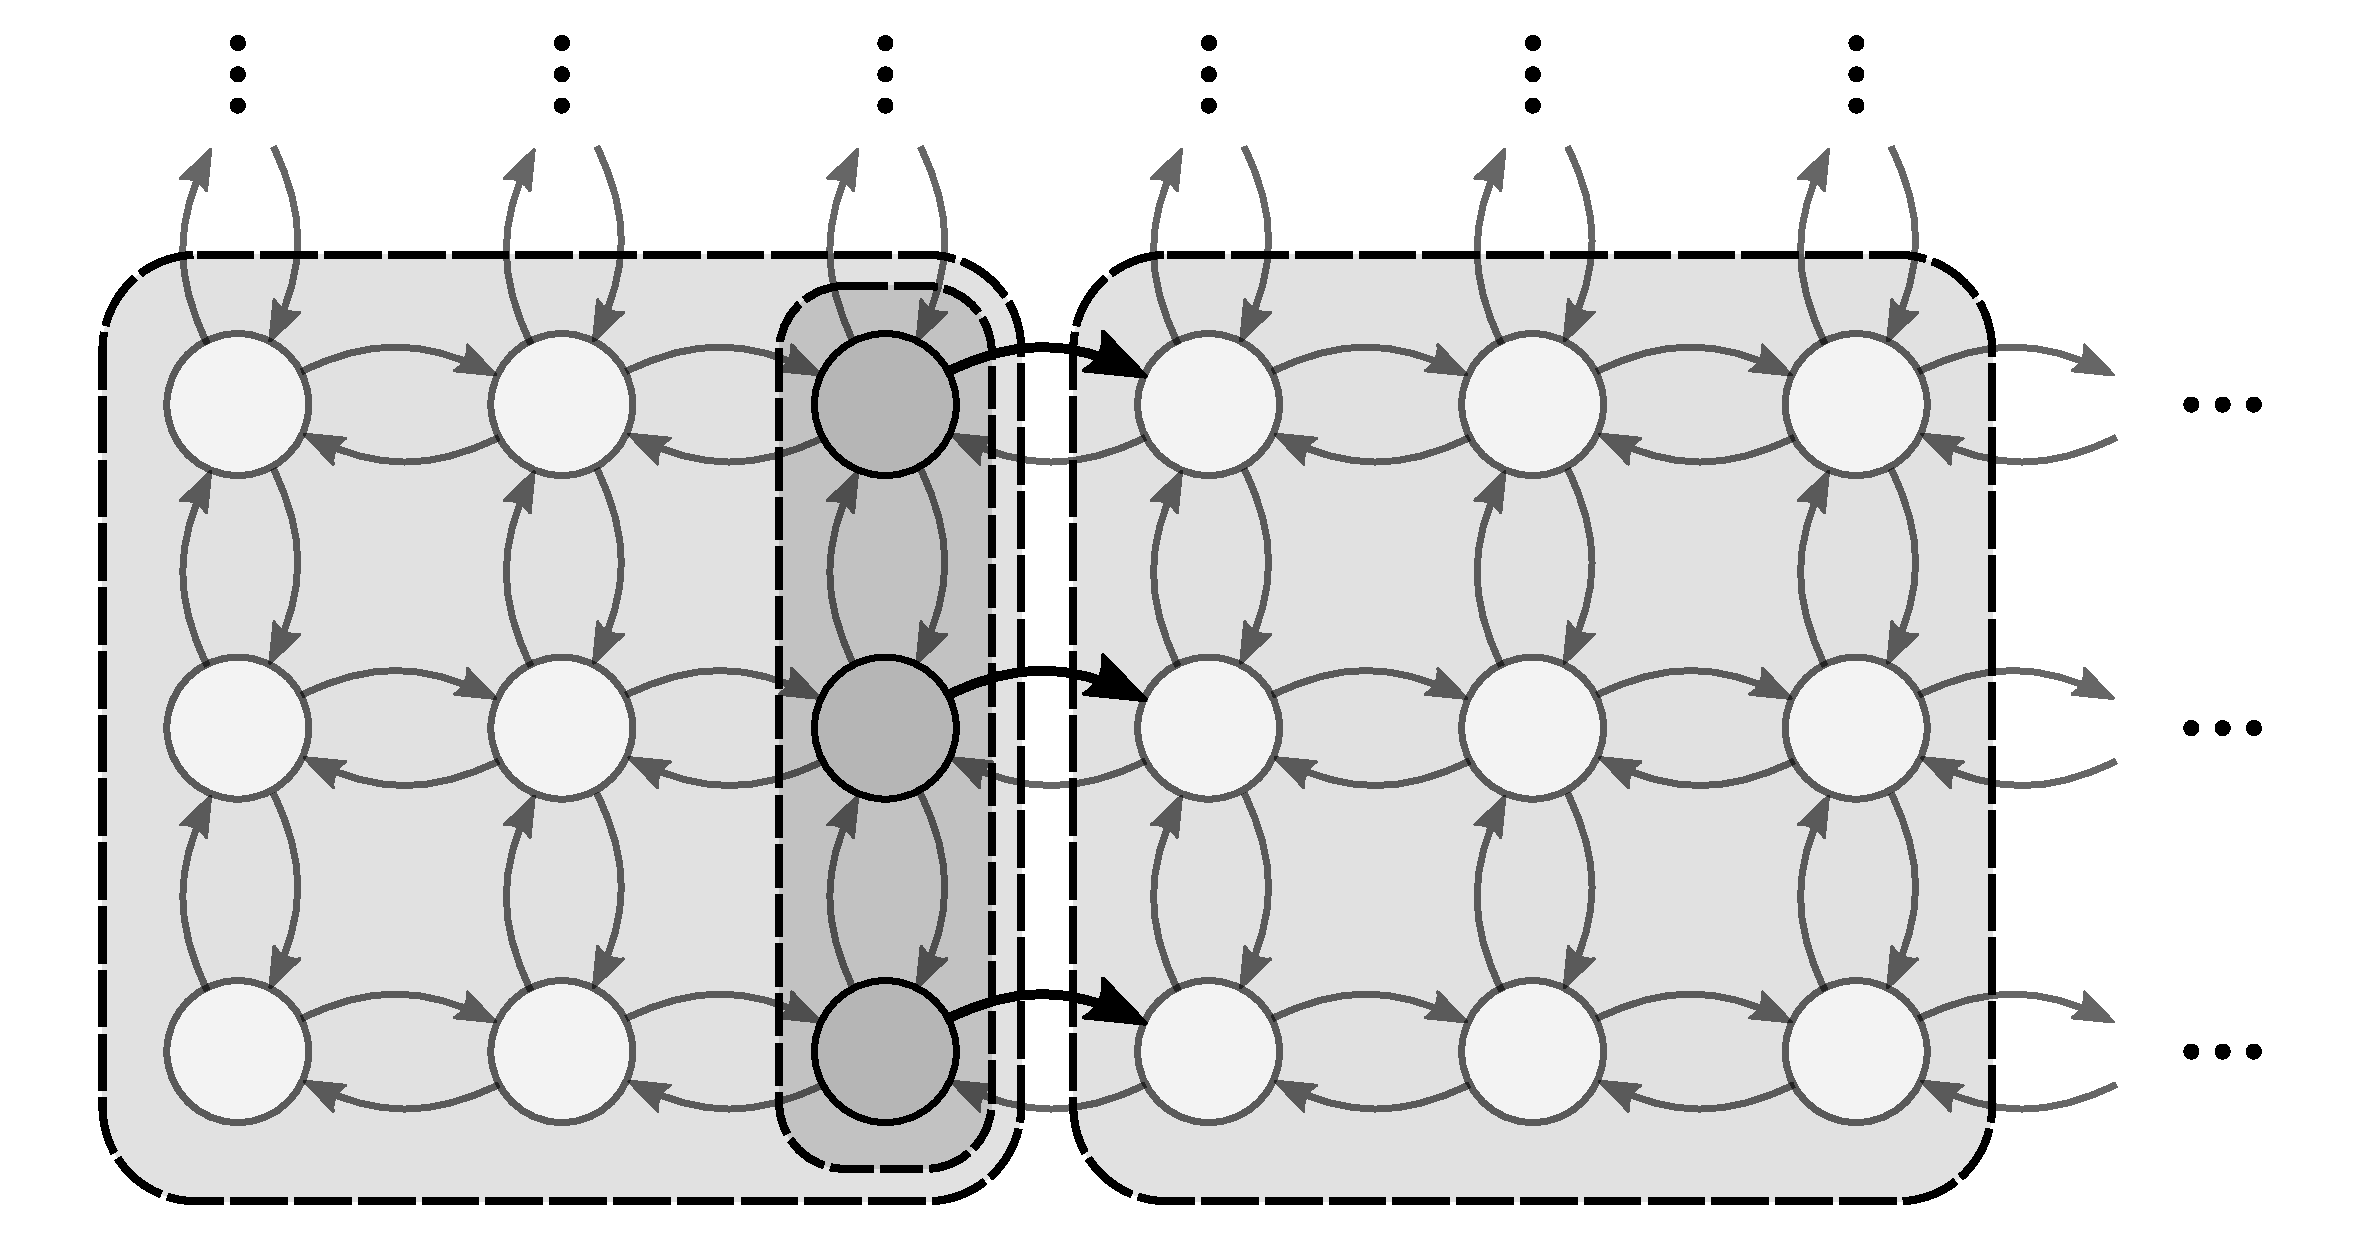
\includegraphics[width=0.9\textwidth]{gfx/macro_states.pdf}
	\caption[Macro-state transition]{\label{fig:macro_states}Two macro-states and a transition state from the left to the right.}
\end{figure}
\end{example}

This uniformity assumption gives rise to the following $Q$-matrix of the aggregated model:
\begin{equation}\label{eq:lumped_q}
    \bar{Q}_{ \bar{x}_i,  \bar{x}_k} = \begin{cases}
        \sum_{j=1}^{n_R}{\bar\alpha}_j\left(\bar{x}_{i\xrightarrow{j}k}\right)/\left|\bar{x}_i\right|\,,&\text{if}\; \bar{x}_i\neq \bar{x}_k\\[1ex]
        -\sum_{j=1}^{n_R}{\bar\alpha}_j\left(\bar{x}_{i\xrightarrow{j}}\right)/{\left|\bar{x}_i\right|}\,, &\text{otherwise}
    \end{cases}
\end{equation}
where 
\begin{equation}\label{eq:lumped_propfun}
    \bar{\alpha}_j({\bar{x}}) = \sum_{x\in \bar{x}} \alpha_j(x).
\end{equation}
is the sum of all rates belonging to reaction $j$ in $\bar{x}$.
In particular, the division by $\left|\bar{x}_i\right|$ in \eqref{eq:lumped_q} is due to the uniformity assumption: According to the assumption, given the process is in $\bar{x}_i$ it is in
each constituent micro-state of the transition state $\bar{x}_{i\xrightarrow{j} k}$ with probability $1/{\left|\bar{x}_i\right|}$.
Therefore, each of the added micro-state rates in \eqref{eq:lumped_propfun} is divided
by the state volume $\left|\bar{x}_i\right|$.

Under the assumption of polynomial rates, as is the case for mass-action
systems, we can compute the sum of rates over this transition set
efficiently using Faulhaber's formula.
\begin{example}
Consider the following mass-action reaction
$ 2 X \xrightarrow{c} \varnothing\,. $
For macro-state
$\bar{x} = \{0, \dots, n\}$
we can compute the corresponding lumped transition rate
\begin{align*}
	\bar{\alpha}(\bar{x})
	& =\frac{c}{2}\sum_{i=1}^n i (i - 1) 
	=\frac{c}{2}\left(\sum_{i=1}^n i^2 - \sum_{i=1}^ni\right)\\
	& =\frac{c}{2}\left(\frac{2n^3+3n^2+n}{6} - \frac{n^2 + n}{2}\right)
\end{align*}
eliminating the explicit summation in the lumped propensity function.
\end{example}

Interestingly, the lumped distribution
tends to be less concentrated. %\MB{rephrase this passage in terms of entropy?}\todo{L: this is interesting, but why? maybe an intuition of why uniform spreads more the distribution}
This is due to the assumption of a
uniform distribution inside macro-states.
This effect is illustrated by the example of a birth-death process below.
Due to this effect, an iterative refinement typically keeps an over-approximation in terms of state-space area.
This is a desirable feature since relevant regions are less likely to be pruned due to lumping approximations.

\begin{example}
We illustrate the scheme on the birth-death process, i.e.\ \autoref{model:bd}.
Its \ac{CTMC} has the following generator matrix
\[
	Q = \begin{bmatrix}
		-\mu & \mu & 0 & & & &\cdots \\
		\gamma & -(\mu + \gamma) & \mu & 0 & && \cdots\\
		0 & 2 \gamma & -(\mu + 2\gamma) & \mu & 0 && \cdots \\
		0 & 0 & 3\gamma & -(\mu + 3\gamma) & \mu &0&\cdots \\
		\vdots & \vdots & \vdots & \vdots & \vdots & \vdots&\ddots
	\end{bmatrix}
\]
The structure is more obvious in the graph visualization:
\vspace{2em}\\
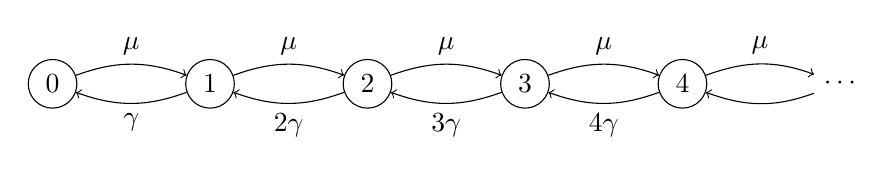
\begin{tikzpicture}{thick}
	\node (n0) at (0, 0) [shape=circle, draw] {$0$};
	\node (n1) at (2, 0) [shape=circle, draw] {$1$};
	\node (n2) at (4, 0) [shape=circle, draw] {$2$};
	\node (n3) at (6, 0) [shape=circle, draw] {$3$};
	\node (n4) at (8, 0) [shape=circle, draw] {$4$};
	\node (n5) at (10, 0) {$\cdots$};
	
	\draw[->] (n0) edge[out=20, in=-200] node[above] {$\mu$} (n1);
	\draw[->] (n1) edge[out=20, in=-200] node[above] {$\mu$} (n2);
	\draw[->] (n2) edge[out=20, in=-200] node[above] {$\mu$} (n3);
	\draw[->] (n3) edge[out=20, in=-200] node[above] {$\mu$} (n4);
	\draw[->] (n4) edge[out=20, in=-200] node[above] {$\mu$} (n5);

	\draw[<-] (n0) edge[out=-20, in=-160] node[below] {$  \gamma$} (n1);
	\draw[<-] (n1) edge[out=-20, in=-160] node[below] {$2 \gamma$} (n2);
	\draw[<-] (n2) edge[out=-20, in=-160] node[below] {$3 \gamma$} (n3);
	\draw[<-] (n3) edge[out=-20, in=-160] node[below] {$4 \gamma$} (n4);
	\draw[<-] (n4) edge[out=-20, in=-160] (n5);
\end{tikzpicture}
\vspace{2em}\\
Now we lump states in groups of $5$ states.
	The states are constructed as\marginpar{We omit the vector notation here for clarity because the process has a single dimension.}
	\[
		\bar{x}_k(5k, (5+1)k - 1)
	\]
	The transition states for the birth reaction $\varnothing\rightarrow S$ is
	\[
		\bar{x}_{k\xrightarrow{1} k+1}=\{5(k+1) -1 \}\,.
	\]
	The lumped transition rate 
	\[
		\bar{\alpha}_1\left(\bar{x}_{k\xrightarrow{1} k+1}\right) = \mu\,.
	\]
	Similarly, the transition states for the death reaction $S\rightarrow \varnothing$ is
	\[
		\bar{x}_{k\xrightarrow{2} k+1}=\{5(k+1)\}\,.
	\]
	The lumped transition rate 
	\[
		\bar{\alpha}_2\left(\bar{x}_{k+1\xrightarrow{1} k}\right) = 5k\gamma\,.
	\]
	Using \eqref{eq:lumped_q} the aggregated transitions are as follows.
\vspace{2em}\\
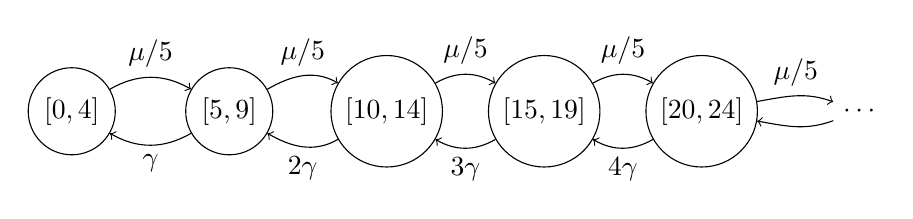
\begin{tikzpicture}{thick}
	\node (n0) at (0, 0) [shape=circle, draw] {$[0,4]$};
	\node (n1) at (2, 0) [shape=circle, draw] {$[5,9]$};
	\node (n2) at (4, 0) [shape=circle, draw] {$[10,14]$};
	\node (n3) at (6, 0) [shape=circle, draw] {$[15,19]$};
	\node (n4) at (8, 0) [shape=circle, draw] {$[20,24]$};
	\node (n5) at (10, 0) {$\cdots$};
	
	\draw[->] (n0) edge[out=30, in=-210] node[above] {$\mu/5$} (n1);
	\draw[->] (n1) edge[out=30, in=-210] node[above] {$\mu/5$} (n2);
	\draw[->] (n2) edge[out=30, in=-210] node[above] {$\mu/5$} (n3);
	\draw[->] (n3) edge[out=30, in=-210] node[above] {$\mu/5$} (n4);
	\draw[->] (n4) edge[out=10, in=-200] node[above] {$\mu/5$} (n5);

	\draw[<-] (n0) edge[out=-30, in=-150] node[below] {$  \gamma$} (n1);
	\draw[<-] (n1) edge[out=-30, in=-150] node[below] {$2 \gamma$} (n2);
	\draw[<-] (n2) edge[out=-30, in=-150] node[below] {$3 \gamma$} (n3);
	\draw[<-] (n3) edge[out=-30, in=-150] node[below] {$4 \gamma$} (n4);
	\draw[<-] (n4) edge[out=-10, in=-160] (n5);
\end{tikzpicture}
In this example the rates remain in effect the same.
But the same number of macro-states covers more micro-states.

A forward integration\marginpar{The integration is done using an ad-hoc \ac{FSP} on $[0, 200]$.} of both, the model at original granularity and the aggregated version
is shown in \autoref{fig:lumped}.
\begin{figure}[htb]
    \centering
    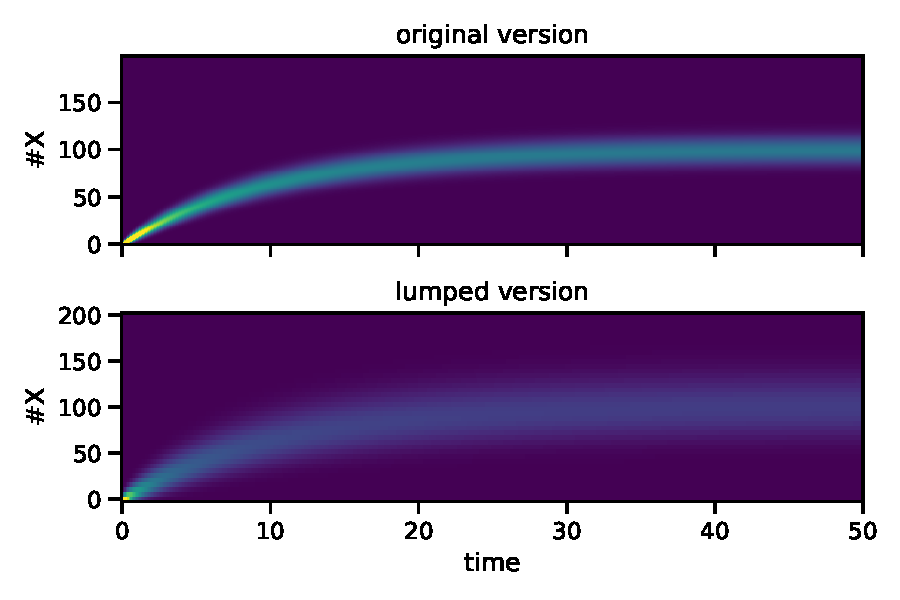
\includegraphics[scale=.6]{gfx/lumpedvorig.pdf}
	\caption[Lumping approximation of \autoref{model:bd}]{A lumping approximation of \autoref{model:bd} on the state-space truncation to $[0, 200]$ on $t\in[0, 50]$. On the left-hand side solutions of a regular truncation approximation and a lumped truncation (macro-state size is $5$) are given.}
    \label{fig:lumped}
\end{figure}
% \begin{figure}[htb]
%     \centering
%     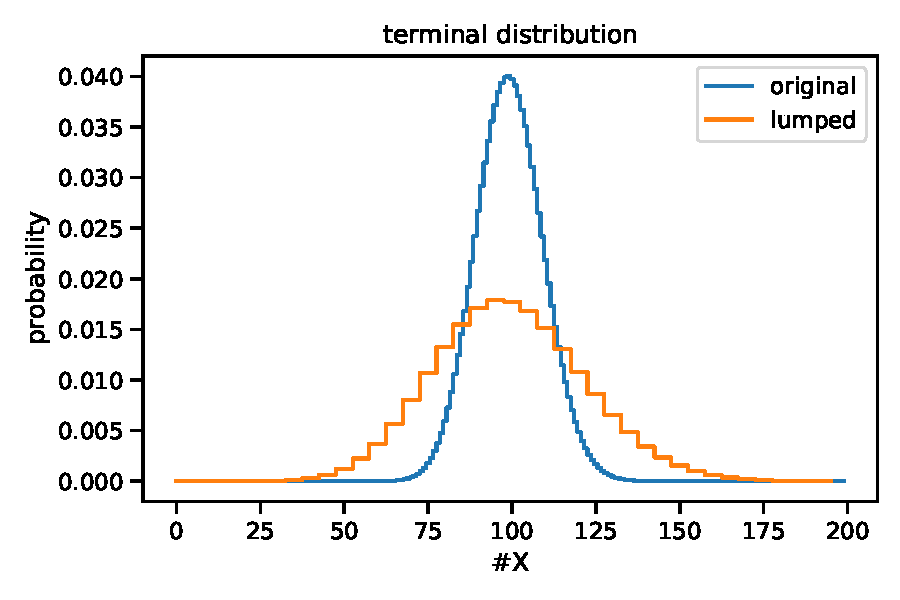
\includegraphics[scale=.6]{gfx/lumped_dist.pdf}
% 	\caption[Distribution of a lumped approximation]{The terminal distributions $\Pr(X_{50}=x_i)$ of a lumped approximation and a truncation at original granularity are given.}
%     \label{fig:lumped_terminal}
% \end{figure}
\end{example}

\section{Approximation Features}
Considering the previous example, we observe that the lumped version shows a similar temporal dynamic, but the distributions are spread out more.
This is a desirable feature because it indicates the location of the main probability mass with
significantly less states.

These features are not valid in general and the aggregation scheme remains a heuristic approach.
This is partly due to the \ac{MPM} formalism allowing for arbitrary propensity functions.
One can construct a process such that a significant change in dynamics inside a macro-state would be missed.
Mostly we encounter this phenomenon in models that exhibit a significant change near the zero-boundary for some species.
Examples include the toggle switch with Hill-functions (\autoref{model:hill_toggle}\turnto{model:hill_toggle}) and die-out in epidemics models (\autoref{model:seir}\turnto{model:seir}).
Other cases are rather rare in the standard model repertoire, but some awareness is necessary.

Fortunately, by refining the aggregation down to ``full resolution'', we can gain the guarantees inherent to \ac{FSP}\@.
